\documentclass[]{article}
\usepackage{lmodern}
\usepackage{amssymb,amsmath}
\usepackage{ifxetex,ifluatex}
\usepackage{fixltx2e} % provides \textsubscript
\ifnum 0\ifxetex 1\fi\ifluatex 1\fi=0 % if pdftex
  \usepackage[T1]{fontenc}
  \usepackage[utf8]{inputenc}
\else % if luatex or xelatex
  \ifxetex
    \usepackage{mathspec}
  \else
    \usepackage{fontspec}
  \fi
  \defaultfontfeatures{Ligatures=TeX,Scale=MatchLowercase}
\fi
% use upquote if available, for straight quotes in verbatim environments
\IfFileExists{upquote.sty}{\usepackage{upquote}}{}
% use microtype if available
\IfFileExists{microtype.sty}{%
\usepackage{microtype}
\UseMicrotypeSet[protrusion]{basicmath} % disable protrusion for tt fonts
}{}
\usepackage[margin=1in]{geometry}
\usepackage{hyperref}
\hypersetup{unicode=true,
            pdftitle={QTL analysis of behavioral traits in Diversity Outbred Mice},
            pdfborder={0 0 0},
            breaklinks=true}
\urlstyle{same}  % don't use monospace font for urls
\usepackage{color}
\usepackage{fancyvrb}
\newcommand{\VerbBar}{|}
\newcommand{\VERB}{\Verb[commandchars=\\\{\}]}
\DefineVerbatimEnvironment{Highlighting}{Verbatim}{commandchars=\\\{\}}
% Add ',fontsize=\small' for more characters per line
\usepackage{framed}
\definecolor{shadecolor}{RGB}{248,248,248}
\newenvironment{Shaded}{\begin{snugshade}}{\end{snugshade}}
\newcommand{\KeywordTok}[1]{\textcolor[rgb]{0.13,0.29,0.53}{\textbf{#1}}}
\newcommand{\DataTypeTok}[1]{\textcolor[rgb]{0.13,0.29,0.53}{#1}}
\newcommand{\DecValTok}[1]{\textcolor[rgb]{0.00,0.00,0.81}{#1}}
\newcommand{\BaseNTok}[1]{\textcolor[rgb]{0.00,0.00,0.81}{#1}}
\newcommand{\FloatTok}[1]{\textcolor[rgb]{0.00,0.00,0.81}{#1}}
\newcommand{\ConstantTok}[1]{\textcolor[rgb]{0.00,0.00,0.00}{#1}}
\newcommand{\CharTok}[1]{\textcolor[rgb]{0.31,0.60,0.02}{#1}}
\newcommand{\SpecialCharTok}[1]{\textcolor[rgb]{0.00,0.00,0.00}{#1}}
\newcommand{\StringTok}[1]{\textcolor[rgb]{0.31,0.60,0.02}{#1}}
\newcommand{\VerbatimStringTok}[1]{\textcolor[rgb]{0.31,0.60,0.02}{#1}}
\newcommand{\SpecialStringTok}[1]{\textcolor[rgb]{0.31,0.60,0.02}{#1}}
\newcommand{\ImportTok}[1]{#1}
\newcommand{\CommentTok}[1]{\textcolor[rgb]{0.56,0.35,0.01}{\textit{#1}}}
\newcommand{\DocumentationTok}[1]{\textcolor[rgb]{0.56,0.35,0.01}{\textbf{\textit{#1}}}}
\newcommand{\AnnotationTok}[1]{\textcolor[rgb]{0.56,0.35,0.01}{\textbf{\textit{#1}}}}
\newcommand{\CommentVarTok}[1]{\textcolor[rgb]{0.56,0.35,0.01}{\textbf{\textit{#1}}}}
\newcommand{\OtherTok}[1]{\textcolor[rgb]{0.56,0.35,0.01}{#1}}
\newcommand{\FunctionTok}[1]{\textcolor[rgb]{0.00,0.00,0.00}{#1}}
\newcommand{\VariableTok}[1]{\textcolor[rgb]{0.00,0.00,0.00}{#1}}
\newcommand{\ControlFlowTok}[1]{\textcolor[rgb]{0.13,0.29,0.53}{\textbf{#1}}}
\newcommand{\OperatorTok}[1]{\textcolor[rgb]{0.81,0.36,0.00}{\textbf{#1}}}
\newcommand{\BuiltInTok}[1]{#1}
\newcommand{\ExtensionTok}[1]{#1}
\newcommand{\PreprocessorTok}[1]{\textcolor[rgb]{0.56,0.35,0.01}{\textit{#1}}}
\newcommand{\AttributeTok}[1]{\textcolor[rgb]{0.77,0.63,0.00}{#1}}
\newcommand{\RegionMarkerTok}[1]{#1}
\newcommand{\InformationTok}[1]{\textcolor[rgb]{0.56,0.35,0.01}{\textbf{\textit{#1}}}}
\newcommand{\WarningTok}[1]{\textcolor[rgb]{0.56,0.35,0.01}{\textbf{\textit{#1}}}}
\newcommand{\AlertTok}[1]{\textcolor[rgb]{0.94,0.16,0.16}{#1}}
\newcommand{\ErrorTok}[1]{\textcolor[rgb]{0.64,0.00,0.00}{\textbf{#1}}}
\newcommand{\NormalTok}[1]{#1}
\usepackage{graphicx,grffile}
\makeatletter
\def\maxwidth{\ifdim\Gin@nat@width>\linewidth\linewidth\else\Gin@nat@width\fi}
\def\maxheight{\ifdim\Gin@nat@height>\textheight\textheight\else\Gin@nat@height\fi}
\makeatother
% Scale images if necessary, so that they will not overflow the page
% margins by default, and it is still possible to overwrite the defaults
% using explicit options in \includegraphics[width, height, ...]{}
\setkeys{Gin}{width=\maxwidth,height=\maxheight,keepaspectratio}
\IfFileExists{parskip.sty}{%
\usepackage{parskip}
}{% else
\setlength{\parindent}{0pt}
\setlength{\parskip}{6pt plus 2pt minus 1pt}
}
\setlength{\emergencystretch}{3em}  % prevent overfull lines
\providecommand{\tightlist}{%
  \setlength{\itemsep}{0pt}\setlength{\parskip}{0pt}}
\setcounter{secnumdepth}{0}
% Redefines (sub)paragraphs to behave more like sections
\ifx\paragraph\undefined\else
\let\oldparagraph\paragraph
\renewcommand{\paragraph}[1]{\oldparagraph{#1}\mbox{}}
\fi
\ifx\subparagraph\undefined\else
\let\oldsubparagraph\subparagraph
\renewcommand{\subparagraph}[1]{\oldsubparagraph{#1}\mbox{}}
\fi

%%% Use protect on footnotes to avoid problems with footnotes in titles
\let\rmarkdownfootnote\footnote%
\def\footnote{\protect\rmarkdownfootnote}

%%% Change title format to be more compact
\usepackage{titling}

% Create subtitle command for use in maketitle
\newcommand{\subtitle}[1]{
  \posttitle{
    \begin{center}\large#1\end{center}
    }
}

\setlength{\droptitle}{-2em}

  \title{QTL analysis of behavioral traits in Diversity Outbred Mice}
    \pretitle{\vspace{\droptitle}\centering\huge}
  \posttitle{\par}
    \author{}
    \preauthor{}\postauthor{}
    \date{}
    \predate{}\postdate{}
  

\begin{document}
\maketitle

\begin{verbatim}
## Warning: package 'qtl2' was built under R version 3.4.4
\end{verbatim}

This tutorial will take you through the process of mapping a QTL and
searching for candidate genes.

The data comes from a behavioral study in which Diversity Outbred (DO)
mice were we characterized \emph{283} male and female DO mice using
open-field, light--dark box, tail-suspension and visual-cliff avoidance
tests to generate 38 behavioral measures. We identified several
quantitative trait loci (QTL) for these traits with support intervals
ranging from 1 to 3 Mb in size. These intervals contain relatively few
genes (ranging from 5 to 96). For a majority of QTL, using the founder
allelic effects together with whole genome sequence data, we could
further narrow the positional candidates. Several QTL replicate
previously published loci. Novel loci were also identified for anxiety-
and activity-related traits. Half of the QTLs are associated with
wild-derived alleles, confirming the value to behavioral genetics of
added genetic diversity in the DO. In the presence of wild-alleles we
sometimes observe behaviors that are qualitatively different from the
expected response. Our results demonstrate that high-precision mapping
of behavioral traits can be achieved with moderate numbers of DO
animals, representing a significant advance in our ability to leverage
the mouse as a tool for behavioral genetics

There are two publications associated with these data. These are
\href{https://www.ncbi.nlm.nih.gov/pubmed/24700285}{Recla JM, et al.
(2014) (Mamm Genome 25:211-222)} and
\href{https://www.ncbi.nlm.nih.gov/pubmed/23433259}{Logan RW, et al.
(2014) (Genes Brain Behav 12:424-437)}

\subsection{QTL mapping workflow}\label{qtl-mapping-workflow}

\begin{figure}
\centering
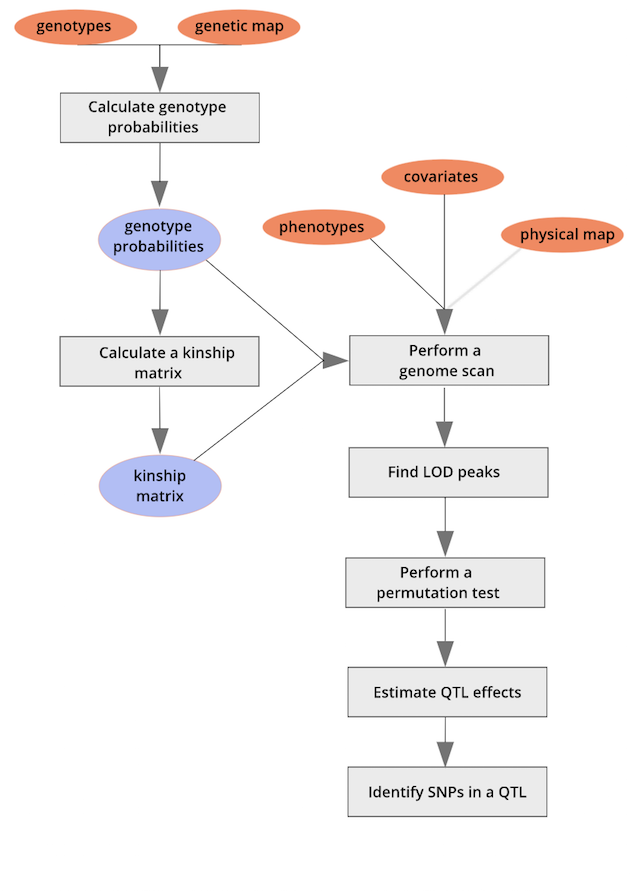
\includegraphics{../figs/mapping-workflow.png}
\caption{}
\end{figure}

\subsubsection{Trait heritability}\label{trait-heritability}

Heritability estimates for the 38 behavioral measurements were
calculated from the progenitor strain data using variance components
from a mixed model with strain as a random effect.
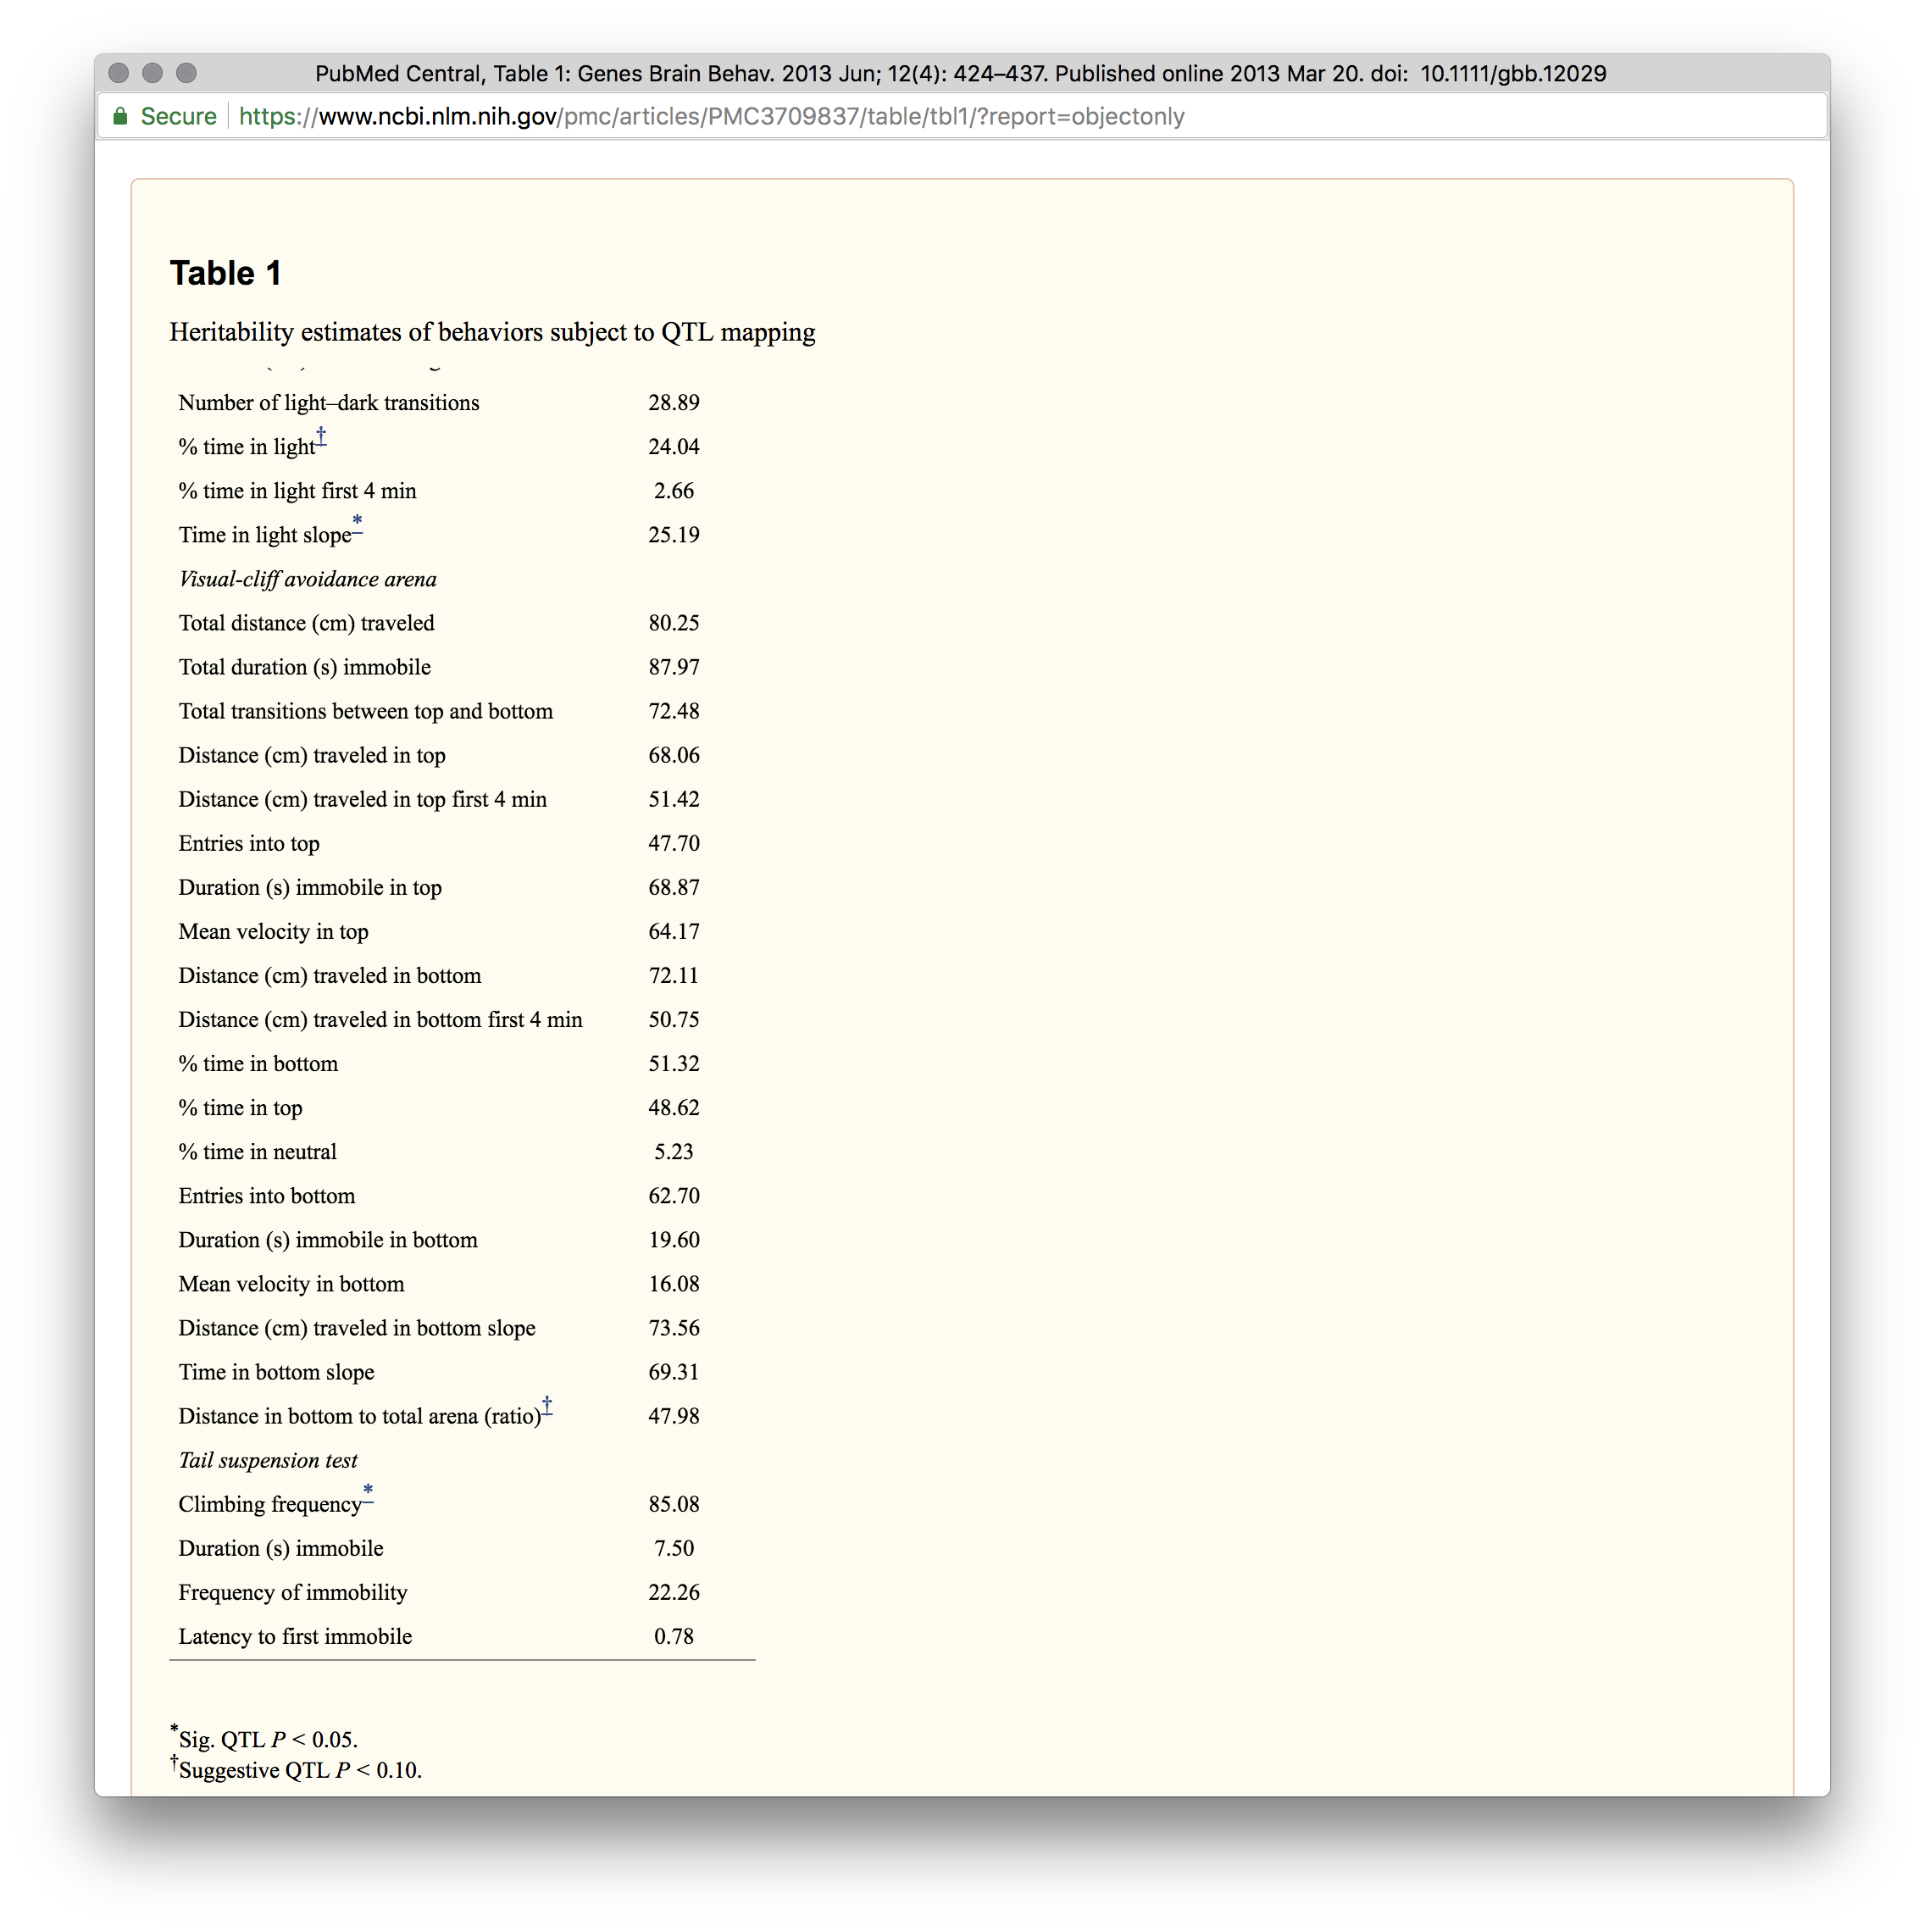
\includegraphics{../figs/Table1_h2.png} Heritabilities can also be
computed on measurements collected using the DO by leveraging the
information containted in the kinship matrix.

\subsubsection{Load and explore the
data}\label{load-and-explore-the-data}

\begin{Shaded}
\begin{Highlighting}[]
\NormalTok{do.cross <-}\StringTok{ }\KeywordTok{read_cross2}\NormalTok{(}\StringTok{"../data/DO_Recla/recla.json"}\NormalTok{)}
\KeywordTok{summary}\NormalTok{(do.cross)}
\end{Highlighting}
\end{Shaded}

\begin{verbatim}
## Object of class cross2 (crosstype "do")
## 
## Total individuals             261
## No. genotyped individuals     261
## No. phenotyped individuals    261
## No. with both geno & pheno    261
## 
## No. phenotypes                 26
## No. covariates                  6
## No. phenotype covariates        0
## 
## No. chromosomes                20
## Total markers                6394
## 
## No. markers by chr:
##   1   2   3   4   5   6   7   8   9  10  11  12  13  14  15  16  17  18 
## 448 447 396 376 359 378 348 305 321 358 314 300 306 306 248 246 216 207 
##  19   X 
## 146 369
\end{verbatim}

\paragraph{The Marker Map}\label{the-marker-map}

The markers are from a genotyping array called the Mouse Universal
Genotyping Array (MUGA) and contains 7,856 SNP markers. Marker locations
for the MUGA and other mouse arrays are available from
\href{ftp://ftp.jax.org/MUGA}{The Jackson Laboratory's FTP site}.

\paragraph{Phenotype distributions}\label{phenotype-distributions}

\textbf{Open field (OF)}
\includegraphics{logan_doqtl_files/figure-latex/plot_phenotypes_OF-1.pdf}

\textbf{Light Dark (LD)}
\includegraphics{logan_doqtl_files/figure-latex/plot_phenotypes_LD-1.pdf}

\textbf{Tail Suspension Test (TST)}
\includegraphics{logan_doqtl_files/figure-latex/plot_phenotypes_TST-1.pdf}

\subsection{QTL mapping of percentage of time spent in the
light}\label{qtl-mapping-of-percentage-of-time-spent-in-the-light}

\begin{figure}
\centering
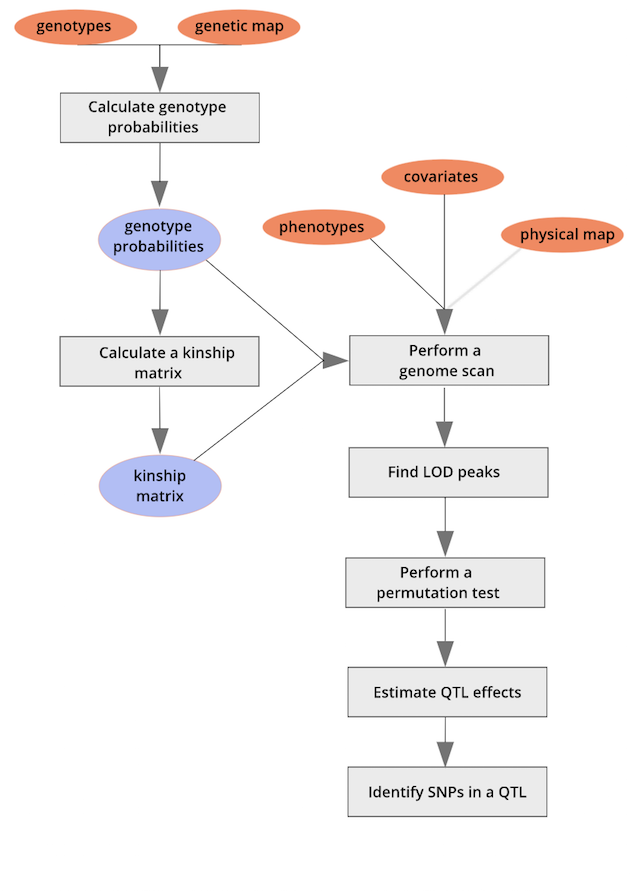
\includegraphics{../figs/mapping-workflow.png}
\caption{}
\end{figure}

\paragraph{\texorpdfstring{\textbf{Genotype (allele)
probabilities}}{Genotype (allele) probabilities}}\label{genotype-allele-probabilities}

\begin{Shaded}
\begin{Highlighting}[]
\NormalTok{n_cores <-}\StringTok{ }\DecValTok{8}
\NormalTok{probs <-}\StringTok{ }\KeywordTok{calc_genoprob}\NormalTok{(do.cross, }\DataTypeTok{error_prob=}\FloatTok{0.002}\NormalTok{, }\DataTypeTok{map_function=}\StringTok{"c-f"}\NormalTok{, }\DataTypeTok{cores=}\NormalTok{n_cores)}
\end{Highlighting}
\end{Shaded}

We now convert the genotype probabilities to haplotype dosages.

\begin{Shaded}
\begin{Highlighting}[]
\NormalTok{aprobs <-}\StringTok{ }\KeywordTok{genoprob_to_alleleprob}\NormalTok{(probs, }\DataTypeTok{cores=}\NormalTok{n_cores)}
\end{Highlighting}
\end{Shaded}

A closer look at the \textbf{eight} haplotypes for just the Chr 1
markers and couple of the DO mice.

\includegraphics{logan_doqtl_files/figure-latex/sample1-1.pdf}
\includegraphics{logan_doqtl_files/figure-latex/sample1-2.pdf}

\includegraphics{logan_doqtl_files/figure-latex/sample10-1.pdf}
\includegraphics{logan_doqtl_files/figure-latex/sample10-2.pdf}

\paragraph{\texorpdfstring{\textbf{Calculate a kinship
matrix}}{Calculate a kinship matrix}}\label{calculate-a-kinship-matrix}

\begin{Shaded}
\begin{Highlighting}[]
\NormalTok{kinship <-}\StringTok{ }\KeywordTok{calc_kinship}\NormalTok{(aprobs, }\StringTok{"loco"}\NormalTok{, }\DataTypeTok{cores=}\NormalTok{n_cores)}
\CommentTok{#kinship <- calc_kinship(aprobs, "overall", cores=n_cores)}

\KeywordTok{image}\NormalTok{(}\DecValTok{1}\OperatorTok{:}\KeywordTok{nrow}\NormalTok{(kinship[[}\DecValTok{1}\NormalTok{]]), }\DecValTok{1}\OperatorTok{:}\KeywordTok{ncol}\NormalTok{(kinship[[}\DecValTok{1}\NormalTok{]]), kinship[[}\DecValTok{1}\NormalTok{]][,}\KeywordTok{ncol}\NormalTok{(kinship[[}\DecValTok{1}\NormalTok{]])}\OperatorTok{:}\DecValTok{1}\NormalTok{], }\DataTypeTok{xlab =} \StringTok{"Samples"}\NormalTok{, }
      \DataTypeTok{ylab =} \StringTok{"Samples"}\NormalTok{, }\DataTypeTok{yaxt =} \StringTok{"n"}\NormalTok{, }\DataTypeTok{main =} \StringTok{"Kinship between samples"}\NormalTok{, }
      \DataTypeTok{breaks =} \DecValTok{0}\OperatorTok{:}\DecValTok{100}\OperatorTok{/}\DecValTok{100}\NormalTok{, }\DataTypeTok{col =} \KeywordTok{heat.colors}\NormalTok{(}\KeywordTok{length}\NormalTok{(}\DecValTok{0}\OperatorTok{:}\DecValTok{100}\NormalTok{) }\OperatorTok{-}\StringTok{ }\DecValTok{1}\NormalTok{))}
\end{Highlighting}
\end{Shaded}

\includegraphics{logan_doqtl_files/figure-latex/calc_kinship-1.pdf}

\begin{Shaded}
\begin{Highlighting}[]
\CommentTok{#image(1:nrow(kinship), 1:ncol(kinship), kinship[,ncol(kinship):1], xlab = "Samples", }
\CommentTok{#      ylab = "Samples", yaxt = "n", main = "Kinship between samples", }
\CommentTok{#      breaks = 0:100/100, col = heat.colors(length(0:100) - 1))}
\end{Highlighting}
\end{Shaded}

The figure above shows kinship between all pairs of samples. White ( =
1) indicates no kinship and red ( = 0) indicates full kinship. Orange
values indicate varying levels of kinship between 0 and 1. The white
diagonal of the matrix indicates that each sample is identical to
itself. The lighter yellow blocks off of the diagonal may indicate
siblings or cousins.

\paragraph{\texorpdfstring{\textbf{Covariates}}{Covariates}}\label{covariates}

\includegraphics{logan_doqtl_files/figure-latex/explore_covar-1.pdf}
\includegraphics{logan_doqtl_files/figure-latex/explore_covar-2.pdf}
\includegraphics{logan_doqtl_files/figure-latex/explore_covar-3.pdf}
\includegraphics{logan_doqtl_files/figure-latex/explore_covar-4.pdf}
\includegraphics{logan_doqtl_files/figure-latex/explore_covar-5.pdf}
\includegraphics{logan_doqtl_files/figure-latex/explore_covar-6.pdf}

\paragraph{\texorpdfstring{\textbf{Including covariates in the mapping
model}}{Including covariates in the mapping model}}\label{including-covariates-in-the-mapping-model}

\begin{Shaded}
\begin{Highlighting}[]
\NormalTok{addcovar =}\StringTok{ }\KeywordTok{model.matrix}\NormalTok{(}\OperatorTok{~}\NormalTok{ngen}\OperatorTok{+}\NormalTok{Group, }\DataTypeTok{data =}\NormalTok{ TS.pheno)[,}\OperatorTok{-}\DecValTok{1}\NormalTok{]}
\end{Highlighting}
\end{Shaded}

\paragraph{\texorpdfstring{\textbf{Running a
genomescan}}{Running a genomescan}}\label{running-a-genomescan}

Before we run the mapping function, let's look at the mapping model. At
each marker on the genotyping array, we will fit a model that regresses
the phenotype \emph{LD\_light\_pct} on covariates and the founder allele
probabilities.

\begin{figure}
\centering
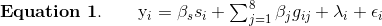
\includegraphics{../figs/equation1.png}
\caption{}
\end{figure}

where:

yi is the phenotype for mouse i,

βs is the effect of study cohort,

si is the study cohort for mouse i,

βj is the effect of founder allele j,

gij is the probability that mouse i carries an allele from founder j,

λi is an adjustment for kinship-induced correlated errors for mouse i,

εi is the residual error for mouse i.

Note that this model will give us an estimate of the effect of each
founder allele at each marker. There are eight founder strains that
contributed to the DO, so we will get eight founder allele effects.

In order to map LD\_light\_pct, you will use the
\href{https://github.com/rqtl/qtl2/blob/master/R/plot_scan1.R}{scan1}
function. To see the arguments for
\href{https://github.com/rqtl/qtl2/blob/master/R/plot_scan1.R}{scan1},
you can type \texttt{help(scan1)}. First, let's map the
\emph{untransformed} phenotype.

\begin{Shaded}
\begin{Highlighting}[]
\NormalTok{index =}\StringTok{ }\KeywordTok{which}\NormalTok{(}\KeywordTok{colnames}\NormalTok{(pheno) }\OperatorTok{==}\StringTok{ "TS_frequency_climbing"}\NormalTok{)}
\NormalTok{qtl.climb =}\StringTok{ }\KeywordTok{scan1}\NormalTok{(}\DataTypeTok{genoprobs =}\NormalTok{ aprobs, }\DataTypeTok{pheno =}\NormalTok{ pheno[,index, }\DataTypeTok{drop =} \OtherTok{FALSE}\NormalTok{], }\DataTypeTok{kinship =}\NormalTok{ kinship, }\DataTypeTok{addcovar =}\NormalTok{ addcovar)}
\end{Highlighting}
\end{Shaded}

Plot of the results, all in gray except for the trait with the largest
LOD score, in blue.

\begin{Shaded}
\begin{Highlighting}[]
\KeywordTok{plot_scan1}\NormalTok{(}\DataTypeTok{x =}\NormalTok{ qtl.climb, }\DataTypeTok{map =}\NormalTok{ do.cross}\OperatorTok{$}\NormalTok{pmap, }\DataTypeTok{main =} \StringTok{"Climbing frequency"}\NormalTok{)}
\end{Highlighting}
\end{Shaded}

\includegraphics{logan_doqtl_files/figure-latex/plot_scan1_TS_frequency_climbing-1.pdf}

\paragraph{Performing a permutation
test}\label{performing-a-permutation-test}

There is resonably large peak on Chr 6, with two additional peaks on Chr
14 and chr 16. Next, we must assess its statistical significance. This
is most commonly done via
\href{http://www.genetics.org/content/178/1/609.long}{permutation}. We
advise running at least 1,000 permutations to obtain significance
thresholds. In the interest of time, we perform 500 permutations here.

\begin{Shaded}
\begin{Highlighting}[]
\NormalTok{perms =}\StringTok{ }\KeywordTok{scan1perm}\NormalTok{(}\DataTypeTok{genoprobs =}\NormalTok{ aprobs, }\DataTypeTok{pheno =}\NormalTok{ pheno[,index, }\DataTypeTok{drop =} \OtherTok{FALSE}\NormalTok{], }\DataTypeTok{addcovar =}\NormalTok{ addcovar, }\DataTypeTok{n_perm =} \DecValTok{100}\NormalTok{)}
\end{Highlighting}
\end{Shaded}

The \texttt{perms} object contains the maximum LOD score from each
genome scan of permuted data.

We can now add thresholds to the previous QTL plot. We use a
significance threshold of p \textless{} 0.05. To do this, we select the
95th percentile of the permutation LOD distribution.

\begin{Shaded}
\begin{Highlighting}[]
\KeywordTok{plot}\NormalTok{(}\DataTypeTok{x =}\NormalTok{ qtl.climb, }\DataTypeTok{map =}\NormalTok{ do.cross}\OperatorTok{$}\NormalTok{pmap,  }\DataTypeTok{main =} \StringTok{"Climbing frequency"}\NormalTok{)}
\NormalTok{thr95 =}\StringTok{ }\KeywordTok{summary}\NormalTok{(perms, }\DataTypeTok{alpha =} \FloatTok{0.05}\NormalTok{)}
\NormalTok{thr90 =}\StringTok{ }\KeywordTok{summary}\NormalTok{(perms, }\DataTypeTok{alpha =} \FloatTok{0.10}\NormalTok{)}
\NormalTok{thr63 =}\StringTok{ }\KeywordTok{summary}\NormalTok{(perms, }\DataTypeTok{alpha =} \FloatTok{0.63}\NormalTok{)}
\KeywordTok{abline}\NormalTok{(}\DataTypeTok{h =} \KeywordTok{c}\NormalTok{(thr95), }\DataTypeTok{col =} \StringTok{"red"}\NormalTok{, }\DataTypeTok{lwd =} \DecValTok{2}\NormalTok{)}
\KeywordTok{abline}\NormalTok{(}\DataTypeTok{h =} \KeywordTok{c}\NormalTok{(thr90), }\DataTypeTok{col =} \StringTok{"red"}\NormalTok{, }\DataTypeTok{lwd =} \DecValTok{1}\NormalTok{)}
\KeywordTok{abline}\NormalTok{(}\DataTypeTok{h =} \KeywordTok{c}\NormalTok{(thr63), }\DataTypeTok{col =} \StringTok{"red"}\NormalTok{, }\DataTypeTok{lwd =} \DecValTok{3}\NormalTok{)}
\end{Highlighting}
\end{Shaded}

\includegraphics{logan_doqtl_files/figure-latex/qtl_plot_thr-1.pdf}

The peak on Chr 6 is above the red significance line. \#\#\#\# Finding
LOD peaks We can then plot the QTL scan. Note that you must provide the
marker map, which we loaded earlier in the MUGA SNP data.

We can find all of the peaks above the significance threshold using the
\href{https://github.com/rqtl/qtl2/blob/master/R/find_peaks.R}{find\_peaks}
function.

\begin{Shaded}
\begin{Highlighting}[]
\KeywordTok{find_peaks}\NormalTok{(}\DataTypeTok{scan1_output =}\NormalTok{ qtl.climb, }\DataTypeTok{map =}\NormalTok{ do.cross}\OperatorTok{$}\NormalTok{pmap, }\DataTypeTok{threshold =}\NormalTok{ thr63)}
\end{Highlighting}
\end{Shaded}

\begin{verbatim}
##   lodindex             lodcolumn chr      pos      lod
## 1        1 TS_frequency_climbing   6 97.82398 7.996058
## 2        1 TS_frequency_climbing  14 36.65222 6.682980
## 3        1 TS_frequency_climbing  18  4.33063 6.320311
\end{verbatim}

The support interval is determined using the
\href{http://www.ncbi.nlm.nih.gov/pubmed/11560912}{Bayesian Credible
Interval} and represents the region most likely to contain the causative
polymorphism(s). We can obtain this interval by adding a \texttt{prob}
argument to
\href{https://github.com/rqtl/qtl2/blob/master/R/find_peaks.R}{find\_peaks}.
We pass in a value of \texttt{0.95} to request a support interval that
contains the causal SNP 95\% of the time.

\begin{Shaded}
\begin{Highlighting}[]
\KeywordTok{find_peaks}\NormalTok{(}\DataTypeTok{scan1_output =}\NormalTok{ qtl.climb, }\DataTypeTok{map =}\NormalTok{ do.cross}\OperatorTok{$}\NormalTok{pmap, }\DataTypeTok{threshold =}\NormalTok{ thr90, }\DataTypeTok{prob =} \FloatTok{0.95}\NormalTok{)}
\end{Highlighting}
\end{Shaded}

\begin{verbatim}
##   lodindex             lodcolumn chr      pos      lod    ci_lo    ci_hi
## 1        1 TS_frequency_climbing   6 97.82398 7.996058 95.67409 98.15002
\end{verbatim}

From the output above, you can see that the support interval is 2.48 Mb
wide (95.67 to 98.15 Mb). The location of the maximum LOD score is at
97.82 Mb.

\paragraph{Estimated QTL effects}\label{estimated-qtl-effects}

We will now zoom in on Chr 6 and look at the contribution of each of the
eight founder alleles to the proportion of bone marrow reticulocytes
that were micro-nucleated. Remember, the mapping model above estimates
the effect of each of the eight DO founders. We can plot these effects
(also called `coefficients') across Chr 6 using
\href{https://github.com/rqtl/qtl2/blob/master/R/scan1coef.R}{scan1coef}.

\begin{Shaded}
\begin{Highlighting}[]
\NormalTok{chr =}\StringTok{ }\DecValTok{6}
\NormalTok{coef06 =}\StringTok{ }\KeywordTok{scan1blup}\NormalTok{(}\DataTypeTok{genoprobs =}\NormalTok{ aprobs[,chr], }\DataTypeTok{pheno =}\NormalTok{ pheno[,index, }\DataTypeTok{drop =} \OtherTok{FALSE}\NormalTok{], }\DataTypeTok{kinship =}\NormalTok{ kinship[[chr]], }\DataTypeTok{addcovar =}\NormalTok{ addcovar)}
\end{Highlighting}
\end{Shaded}

This produces an object containing estimates of each of the eight DO
founder allele effect. These are the βj values in the mapping equation
above.

\begin{Shaded}
\begin{Highlighting}[]
\KeywordTok{plot_coefCC}\NormalTok{(}\DataTypeTok{x =}\NormalTok{ coef06, }\DataTypeTok{map =}\NormalTok{ do.cross}\OperatorTok{$}\NormalTok{pmap, }\DataTypeTok{scan1_output =}\NormalTok{ qtl.climb, }\DataTypeTok{main =} \StringTok{"Climbing frequency"}\NormalTok{)}
\end{Highlighting}
\end{Shaded}

\includegraphics{logan_doqtl_files/figure-latex/coef_plot-1.pdf}

The top panel shows the eight founder allele effects (or model
coefficients) along Chr 6. The founder allele effects are centerd at
zero and the units are the same as the phenotype. You can see that DO
mice containing the CAST/EiJ allele near 34 Mb have lower levels of
micro-nucleated reticulocytes. This means that the CAST allele is
associated with less DNA damage and has a protective effect. The bottom
panel shows the LOD score, with the support interval for the peak shaded
blue.

\paragraph{SNP Association Mapping}\label{snp-association-mapping}

At this point, we have a 2.50 Mb wide support interval that contains a
polymorphism(s) that influences benzene-induced DNA damage. Next, we
will impute the DO founder sequences onto the DO genomes. The
\href{http://www.sanger.ac.uk/resources/mouse/genomes/}{Sanger Mouse
Genomes Project} has sequenced the eight DO founders and provides SNP,
insertion-deletion (indel), and structural variant files for the strains
(see
\href{http://www.nature.com/ng/journal/v45/n7/full/ng.2644.html}{Baud
et.al., Nat. Gen., 2013}). We can impute these SNPs onto the DO genomes
and then perform association mapping. The process involves several steps
and I have provided a function to encapsulate the steps. To access the
Sanger SNPs, we use a SQLlite database provided by
\href{https://github.com/kbroman}{Karl Broman}. You should have
downloaded this during \href{../setup.md}{Setup}. It is available from
the \href{ftp://ftp.jax.org/dgatti/CC_SNP_DB/cc_variants.sqlite}{JAX FTP
site}, but the file is 3 GB, so it may take too long to download right
now.

\begin{figure}
\centering
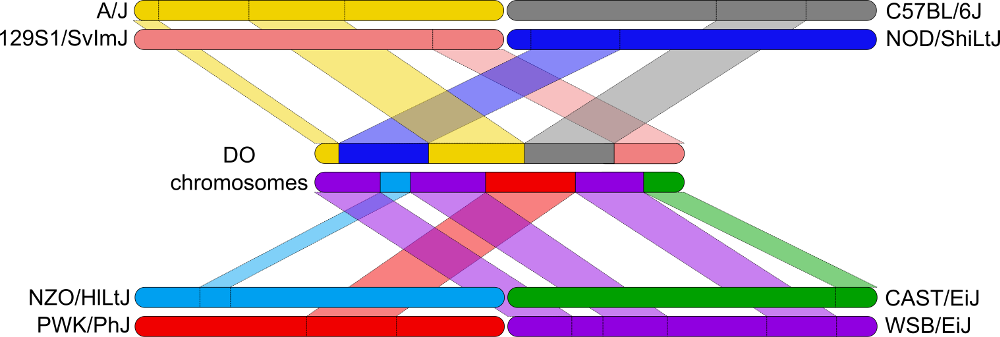
\includegraphics{../figs/DO.impute.founders.sm.png}
\caption{}
\end{figure}

Association mapping involves imputing the founder SNPs onto each DO
genome and fitting the mapping model at each SNP. At each marker, we fit
the following model:

\begin{figure}
\centering
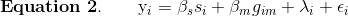
\includegraphics{../figs/equation2.png}
\caption{}
\end{figure}

where:

yi is the phenotype for mouse i,

βs is the effect of study cohort,

si is the study cohort for mouse i,

βm is the effect of adding one allele at marker m,

gim is the allele call for mouse i at marker m,

λi is an adjustment for kinship-induced correlated errors for mouse i,

εi is the residual error for mouse i.

We can call
\href{https://github.com/rqtl/qtl2/blob/master/R/scan1snps.R}{scan1snps}
to perform association mapping in the QTL interval on Chr 6. We first
create variables for the chromosome and support interval where we are
mapping. We then create a function to get the SNPs from the founder SNP
database The path to the SNP database (\texttt{snpdb\_file} argument)
points to the data directory on your computer. Note that it is important
to use the \texttt{keep\_all\_snps\ =\ TRUE} in order to return all
SNPs.

\begin{Shaded}
\begin{Highlighting}[]
\NormalTok{chr =}\StringTok{ }\DecValTok{6}
\NormalTok{start =}\StringTok{ }\DecValTok{95}
\NormalTok{end =}\StringTok{ }\DecValTok{99}
\NormalTok{query_func =}\StringTok{ }\KeywordTok{create_variant_query_func}\NormalTok{(}\StringTok{"../data/cc_variants.sqlite"}\NormalTok{)}
\NormalTok{assoc =}\StringTok{ }\KeywordTok{scan1snps}\NormalTok{(}\DataTypeTok{genoprobs =}\NormalTok{ aprobs[,chr], }\DataTypeTok{map =}\NormalTok{ do.cross}\OperatorTok{$}\NormalTok{pmap, }\DataTypeTok{pheno =}\NormalTok{ pheno[,index,}\DataTypeTok{drop =} \OtherTok{FALSE}\NormalTok{], }\DataTypeTok{kinship =}\NormalTok{ kinship, }\DataTypeTok{addcovar =}\NormalTok{ addcovar, }\DataTypeTok{query_func =}\NormalTok{ query_func, }\DataTypeTok{chr =}\NormalTok{ chr, }\DataTypeTok{start =}\NormalTok{ start, }\DataTypeTok{end =}\NormalTok{ end, }\DataTypeTok{keep_all_snps =} \OtherTok{TRUE}\NormalTok{)}
\end{Highlighting}
\end{Shaded}

The \texttt{assoc} object is a list containing two objects: the LOD
scores for each unique SNP and a \texttt{snpinfo} object that maps the
LOD scores to each SNP. To plot the association mapping, we need to
provide both objects to the
\href{https://github.com/rqtl/qtl2/blob/master/R/plot_snpasso.R}{plot\_snpasso}
function.

\begin{Shaded}
\begin{Highlighting}[]
\KeywordTok{plot_snpasso}\NormalTok{(}\DataTypeTok{scan1output =}\NormalTok{ assoc}\OperatorTok{$}\NormalTok{lod, }\DataTypeTok{snpinfo =}\NormalTok{ assoc}\OperatorTok{$}\NormalTok{snpinfo, }\DataTypeTok{main =} \StringTok{"Climbing frequency"}\NormalTok{)}
\end{Highlighting}
\end{Shaded}

\includegraphics{logan_doqtl_files/figure-latex/assoc_fig-1.pdf}

This plot shows the LOD score for each SNP in the QTL interval. The SNPs
occur in ``shelves'' because all of the SNPs in a haplotype block have
the same founder strain pattern. The SNPs with the highest LOD scores
are the ones for which CAST/EiJ contributes the alternate allele.

We can add a plot containing the genes in the QTL interval using the
\texttt{plot\_genes} function. We get the genes from another SQLlite
database created by \href{https://github.com/kbroman}{Karl Broman}
called \texttt{mouse\_genes.sqlite}. You should have downloaded this
from the
\href{ftp://ftp.jax.org/dgatti/CC_SNP_DB/mouse_genes.sqlite}{JAX FTP
Site} during \href{../setup.md}{Setup}.

First, we must query the database for the genes in the interval. The
path of the first argument points to the data directory on your
computer.

\begin{Shaded}
\begin{Highlighting}[]
\NormalTok{query_genes =}\StringTok{ }\KeywordTok{create_gene_query_func}\NormalTok{(}\DataTypeTok{dbfile =} \StringTok{"../data/mouse_genes.sqlite"}\NormalTok{, }\DataTypeTok{filter =} \StringTok{"source='MGI'"}\NormalTok{)}
\NormalTok{genes =}\StringTok{ }\KeywordTok{query_genes}\NormalTok{(chr, start, end)}
\KeywordTok{head}\NormalTok{(genes)}
\end{Highlighting}
\end{Shaded}

\begin{verbatim}
##   chr source       type    start     stop score strand phase
## 1   6    MGI       gene 95.09201 95.09508    NA   <NA>    NA
## 2   6    MGI       gene 95.10020 95.10031    NA      -    NA
## 3   6    MGI       gene 95.11401 95.11795    NA      -    NA
## 4   6    MGI       gene 95.11724 95.12979    NA      +    NA
## 5   6    MGI pseudogene 95.23992 95.24061    NA      -    NA
## 6   6    MGI pseudogene 95.25030 95.25451    NA      +    NA
##                ID          Name Parent
## 1 MGI:MGI:1920900 2410024F20Rik   <NA>
## 2 MGI:MGI:5456278       Gm26501   <NA>
## 3 MGI:MGI:1919467      Kbtbd8os   <NA>
## 4 MGI:MGI:2661430        Kbtbd8   <NA>
## 5 MGI:MGI:5010007       Gm17822   <NA>
## 6 MGI:MGI:3647796        Gm5723   <NA>
##                                                                   Dbxref
## 1                                                       GenBank:AK010580
## 2                                             ENSEMBL:ENSMUSG00000093999
## 3 VEGA:OTTMUSG00000057788,NCBI_Gene:102634268,ENSEMBL:ENSMUSG00000085413
## 4    VEGA:OTTMUSG00000029697,NCBI_Gene:243574,ENSEMBL:ENSMUSG00000030031
## 5 VEGA:OTTMUSG00000057789,NCBI_Gene:100328567,ENSEMBL:ENSMUSG00000107934
## 6    VEGA:OTTMUSG00000057790,NCBI_Gene:435912,ENSEMBL:ENSMUSG00000107900
##                                                             mgiName
## 1                                        RIKEN cDNA 2410024F20 gene
## 2                                           predicted gene%2c 26501
## 3 kelch repeat and BTB (POZ) domain containing 8%2c opposite strand
## 4                    kelch repeat and BTB (POZ) domain containing 8
## 5                                           predicted gene%2c 17822
## 6                                               predicted gene 5723
##                 bioType Alias
## 1     unclassified gene  <NA>
## 2            snRNA gene  <NA>
## 3 antisense lncRNA gene  <NA>
## 4   protein coding gene  <NA>
## 5            pseudogene  <NA>
## 6            pseudogene  <NA>
\end{verbatim}

The \texttt{genes} object contains annotation information for each gene
in the interval.

Next, we will create a plot with two panels: one containing the
association mapping LOD scores and one containing the genes in the QTL
interval. We do this by passing in the \texttt{genes} argument to
\href{https://github.com/rqtl/qtl2/blob/master/R/plot_snpasso.R}{plot\_snpasso}.

\includegraphics{logan_doqtl_files/figure-latex/plot_assoc2-1.pdf}


\end{document}
